\documentclass[]{book}
\usepackage{lmodern}
\usepackage{amssymb,amsmath}
\usepackage{ifxetex,ifluatex}
\usepackage{fixltx2e} % provides \textsubscript
\ifnum 0\ifxetex 1\fi\ifluatex 1\fi=0 % if pdftex
  \usepackage[T1]{fontenc}
  \usepackage[utf8]{inputenc}
\else % if luatex or xelatex
  \ifxetex
    \usepackage{mathspec}
  \else
    \usepackage{fontspec}
  \fi
  \defaultfontfeatures{Ligatures=TeX,Scale=MatchLowercase}
\fi
% use upquote if available, for straight quotes in verbatim environments
\IfFileExists{upquote.sty}{\usepackage{upquote}}{}
% use microtype if available
\IfFileExists{microtype.sty}{%
\usepackage{microtype}
\UseMicrotypeSet[protrusion]{basicmath} % disable protrusion for tt fonts
}{}
\usepackage{hyperref}
\hypersetup{unicode=true,
            pdftitle={Twitter for Scientists},
            pdfauthor={Daniel S. Quintana},
            pdfborder={0 0 0},
            breaklinks=true}
\urlstyle{same}  % don't use monospace font for urls
\usepackage{natbib}
\bibliographystyle{apalike}
\usepackage{longtable,booktabs}
\usepackage{graphicx,grffile}
\makeatletter
\def\maxwidth{\ifdim\Gin@nat@width>\linewidth\linewidth\else\Gin@nat@width\fi}
\def\maxheight{\ifdim\Gin@nat@height>\textheight\textheight\else\Gin@nat@height\fi}
\makeatother
% Scale images if necessary, so that they will not overflow the page
% margins by default, and it is still possible to overwrite the defaults
% using explicit options in \includegraphics[width, height, ...]{}
\setkeys{Gin}{width=\maxwidth,height=\maxheight,keepaspectratio}
\IfFileExists{parskip.sty}{%
\usepackage{parskip}
}{% else
\setlength{\parindent}{0pt}
\setlength{\parskip}{6pt plus 2pt minus 1pt}
}
\setlength{\emergencystretch}{3em}  % prevent overfull lines
\providecommand{\tightlist}{%
  \setlength{\itemsep}{0pt}\setlength{\parskip}{0pt}}
\setcounter{secnumdepth}{5}
% Redefines (sub)paragraphs to behave more like sections
\ifx\paragraph\undefined\else
\let\oldparagraph\paragraph
\renewcommand{\paragraph}[1]{\oldparagraph{#1}\mbox{}}
\fi
\ifx\subparagraph\undefined\else
\let\oldsubparagraph\subparagraph
\renewcommand{\subparagraph}[1]{\oldsubparagraph{#1}\mbox{}}
\fi

%%% Use protect on footnotes to avoid problems with footnotes in titles
\let\rmarkdownfootnote\footnote%
\def\footnote{\protect\rmarkdownfootnote}

%%% Change title format to be more compact
\usepackage{titling}

% Create subtitle command for use in maketitle
\providecommand{\subtitle}[1]{
  \posttitle{
    \begin{center}\large#1\end{center}
    }
}

\setlength{\droptitle}{-2em}

  \title{Twitter for Scientists}
    \pretitle{\vspace{\droptitle}\centering\huge}
  \posttitle{\par}
    \author{Daniel S. Quintana}
    \preauthor{\centering\large\emph}
  \postauthor{\par}
      \predate{\centering\large\emph}
  \postdate{\par}
    \date{March 4, 2020 (version 0.1)}

\usepackage{booktabs}

\begin{document}
\maketitle

{
\setcounter{tocdepth}{1}
\tableofcontents
}
\hypertarget{preface}{%
\chapter*{Preface}\label{preface}}
\addcontentsline{toc}{chapter}{Preface}

\begin{center}\includegraphics[width=0.5\linewidth]{images/cover} \end{center}

\hypertarget{why-i-wrote-this-book}{%
\section*{Why I wrote this book}\label{why-i-wrote-this-book}}
\addcontentsline{toc}{section}{Why I wrote this book}

There are four ways to get your research known, but only only one of these is an option for every early career researcher:

\begin{enumerate}
\def\labelenumi{\arabic{enumi}.}
\tightlist
\item
  Already be famous
\item
  Have a famous mentor
\item
  Repeatedly win the peer-review lottery
\item
  Actively contribute to social media
\end{enumerate}

I wouldn't still be in academia if it wasn't for Twitter, which is currently the premier social media platform for science communication. Twitter has given me the skills to keep me up-to-date with emerging tools and the networks for advice and research collaboration. I'm writing this book because I believe that Twitter provides incredible opportunities to scientists, regardless of their senority, who their or their mentor is, or thier instution.

The most common question I get at social media workshops that I've organised is, ``What should I tweet?''. There is no easy answer to this, because every researcher and their subfield is different. But there's one core princple that will always point you in the right direction: \emph{the best way to engage your followers is to either entertain or educate}. In other words, you should aim to help people either pass time or save time. Being entertaining doesn't come naturally to most people, so don't worry if this is you. But as a scientist, you are very well-placed to educate, no matter your level of training.

This book will walk you through the nuts and bolts of twitter, and is set at three levels: Beginner, intermediate, and advanced. After the beginner chapter I've put together a one-month challenge, to help you build some momentum with your tweeting.

\hypertarget{a-few-comments-about-this-book}{%
\section*{A few comments about this book}\label{a-few-comments-about-this-book}}
\addcontentsline{toc}{section}{A few comments about this book}

Unless specified otherwise examples and instructions will be using twitter on your desktop brower. There are a few small differences between using Twitter on your desktop browser and using the iOS or Andriod app. However, their similar enough that this book should be transferrable.

When I use Twitter on my desktop browser, I use a blue color theme with a `Lights out' background. This isn't the default scheme, so the screenshots used in this book may look different to how Twitter looks on your desktop. Here's how to change your display settings (Figure \ref{fig:display}).

\begin{figure}

{\centering \includegraphics[width=0.8\linewidth]{images/display} 

}

\caption{Change your desktop display settings by clicking on "More" in your menu bar (1), and then clicking on "dispay" in the Settings menu}\label{fig:display}
\end{figure}

It's worth noting that I've written this guide from my perspective as a researcher in the psychological and biomedical sciences. This means that some things that I mention (e.g., preprints) might not be relevant for your scientific field. Pick and choose what is relevant to your field.

Twitter is constantly in flux. The platform didn't begin with retweets or images, let along threads and GIFs, so many of the examples in this book may not be relevant in the future. New features are constantly tested in smaller worldwide markets. As I'm writing this, I just saw that an ephermel tweet feature, in which there will be a seperate timeline in which tweets will disappear after 24 hours, has just been launched in Brazil. This might disappear as an option for Brazilian Twitter users or could be available for everyone in the coming months.

It's hard to predict what Twitter will look like in the future, however, the broad principles of Twitter should remain the same. I will do my best to update this book in the future, in response to changes in Twitter's platform and norms around how scientists use Twitter.

\hypertarget{about-me}{%
\section*{About me}\label{about-me}}
\addcontentsline{toc}{section}{About me}

I'm a research scientist at the University of Oslo. I was awarded my PhD in Psychology in 2013 at the University of Sydney. I now investigate how the hormone oxytocin influences how we think and feel. I'm also intersted in cardiac psychophysiology and meta-science, which the science of scientific practice. As this is a book about twitter, you will not be suprised to read that I \href{https://twitter.com/dsquintana}{tweet a lot}

I'm the co-host and producer of \href{https://everythinghertz.com/}{\emph{Everything Hertz}}, which is a podcast about methodology and scientific life in the biobehavioral sciences. We talk a lot about Twitter on this show, and many of our discussions are inspired by tweets from other users.

I live on an island in the Oslo fjord with my wife and two daughters.

\hypertarget{beginner}{%
\chapter{An introduction to Twitter}\label{beginner}}

Twitter was was originally conceived as a ``micro-blogging'' platform, in which users posted short text updates, but it later evolved into a social network where users interact. The core of this platform is that users share 280 character text posts, which can include links and other media, like images and videos. It's also easy to add emoji, which can add a little personality to your tweets (Figure \ref{fig:compose}).

\begin{figure}

{\centering \includegraphics[width=0.8\linewidth]{images/compose} 

}

\caption{The compose window when using Twitter in a desktop web browser.}\label{fig:compose}
\end{figure}

\hypertarget{setting-up-your-twitter-profile}{%
\section{Setting up your Twitter profile}\label{setting-up-your-twitter-profile}}

After you've \href{https://twitter.com/}{signed up for an account on Twitter}, you should spend a few moments setting up your profile page. This is important, as people will typically check your profile page before they follow you.

\hypertarget{your-username}{%
\subsection{Your username}\label{your-username}}

If you're still hesitant about joining Twitter, \emph{at least} sign up so that you can secure a good username. The longer you wait before signing up, the less likely you can secure a username to your liking. If possible, try to avoid a long string of numbers at the end of your username, because these types of names are often associated with bot accounts.

If you can, pick username something close to your actual name, as this will make it easier for others to find you. Avoid a username something associated with your current research area---this might change in the future! Shorter names are also better, as these are easier for people to remember and count less towards twitter character limits when other people mention you in their tweets (more on this later). If you have a common name and all the possible permutations of your name are taken, don't worry too much.

Even if you can't get your desired username, you can still use any name you like for your the display name (Figure \ref{fig:profile}).

\begin{figure}

{\centering \includegraphics[width=0.8\linewidth]{images/profile} 

}

\caption{A Twitter profile}\label{fig:profile}
\end{figure}

\hypertarget{your-profile-picture}{%
\subsection{Your profile picture}\label{your-profile-picture}}

It is important that you change your profile picture to something different from the default, is this helps others realise that you're not a bot and also helps people identify you. The most obvious picture to use as a profile image of yourself, but this isn't necessary. It's fine to change your image every now and then, but don't do this too often as people may not recognise you when you tweet.

You can use a JPEG or GIF file with a maximum size of 2MB. As Twitter is used on a range of devices, Twitter recommends that profile photos are 400x400 pixels.

\hypertarget{your-twitter-header-image}{%
\subsection{Your Twitter header image}\label{your-twitter-header-image}}

This is another opportunity for people to get a sense of what to expect when they follow you. If you would like some inspiration, get a free Canva account (\url{https://canva.com/}) and then search ``Twitter Header'' for some free design templates that use the required dimensions (1500 by 500 pixels).

Another common twitter image as a landscape shot of where you live (or where you grew up), an image of you giving a presentation, or an image of your latest publication. There aren't any specific rules here, but use the opportunity to share your personality.

Twitter also has its own \href{https://www.flickr.com/photos/twitteroffice/sets/72157643560484885/}{header image gallery}, with images that are the recommended size.

\hypertarget{your-bio}{%
\subsection{Your bio}\label{your-bio}}

Share a short description of your research area and the sort of thing that people can expect if they follow you. These are limited to 160 characters, which isn't a lot. You may also consider including the twitter handle of the institution you work at in your bio.

Feel free to add emoji to give your bio a little more personality. This can give you a few extra characters that you can use. For instance, rather than saying you're Australian, you can include an emoji of the Australian flag, which saves you a handful of characters. You can also use emoji to highlight your research area. For instance, if you're a neuroscientist you can use a brain emoji.

\hypertarget{the-website-link}{%
\subsection{The website link}\label{the-website-link}}

This is another good opportunity for people to learn about you. As an academic, people want to find out about your publications and your current projects. If you're a scientist you should have your own website, as people \emph{will} Google you. If you have a basic familiarity with R, I've put together an \href{https://www.dsquintana.blog/free-website-in-r-easy/}{easy-to-follow guide}. Other options include your institutional website, or your Google Scholar profile.

\hypertarget{location}{%
\subsection{Location}\label{location}}

It's up to you how specific you want to be when it comes to your location. Adding your city could be helpful, as people may want to contact and meet you in person if they're travelling through your town. You don't have to put

\hypertarget{the-anatomy-of-a-tweet}{%
\section{The anatomy of a tweet}\label{the-anatomy-of-a-tweet}}

Tweets can include text (up to 280 characters), 1-4 images (PNG or JPG), a single GIF, or a video. You can also post both text and one of the types of media described above.

\hypertarget{using-text-in-your-tweets}{%
\subsection{Using text in your tweets}\label{using-text-in-your-tweets}}

Twitter was originally concieved as a SMS-based service, in which you could send text-only tweets via SMS. In fact, this SMS tweet-features \href{https://help.twitter.com/en/using-twitter/twitter-sms}{still exists}. Even today, the majority of tweets are text only, so this is Twitter's bread and butter.

Your text you can also include website URLs. Regardless of the size of the URL, Twitter will treat each URL as 23 characters.

You can also mention other Twitter uses, by writing the `@' symbol, followed by thier twitter username, like this: ``\citet{dsquintana}''

\hypertarget{the-types-of-images-and-videos-you-can-include-with-your-tweets}{%
\subsection{The types of images and videos you can include with your tweets}\label{the-types-of-images-and-videos-you-can-include-with-your-tweets}}

In terms of static images, you can upload JPG and PNG files. Adding images are a nice way to help make your tweets stand out. Photos can be up to 5MB in size.

If you're looking for images to illustrate a tweet, I recommend doing a search on \href{https://unsplash.com/}{unsplash.com}, as you can use these high-quality images without attribution. Here's an example of the kind of image you can find on Unsplash. (Figure \ref{fig:unsplash}).

\begin{figure}

{\centering 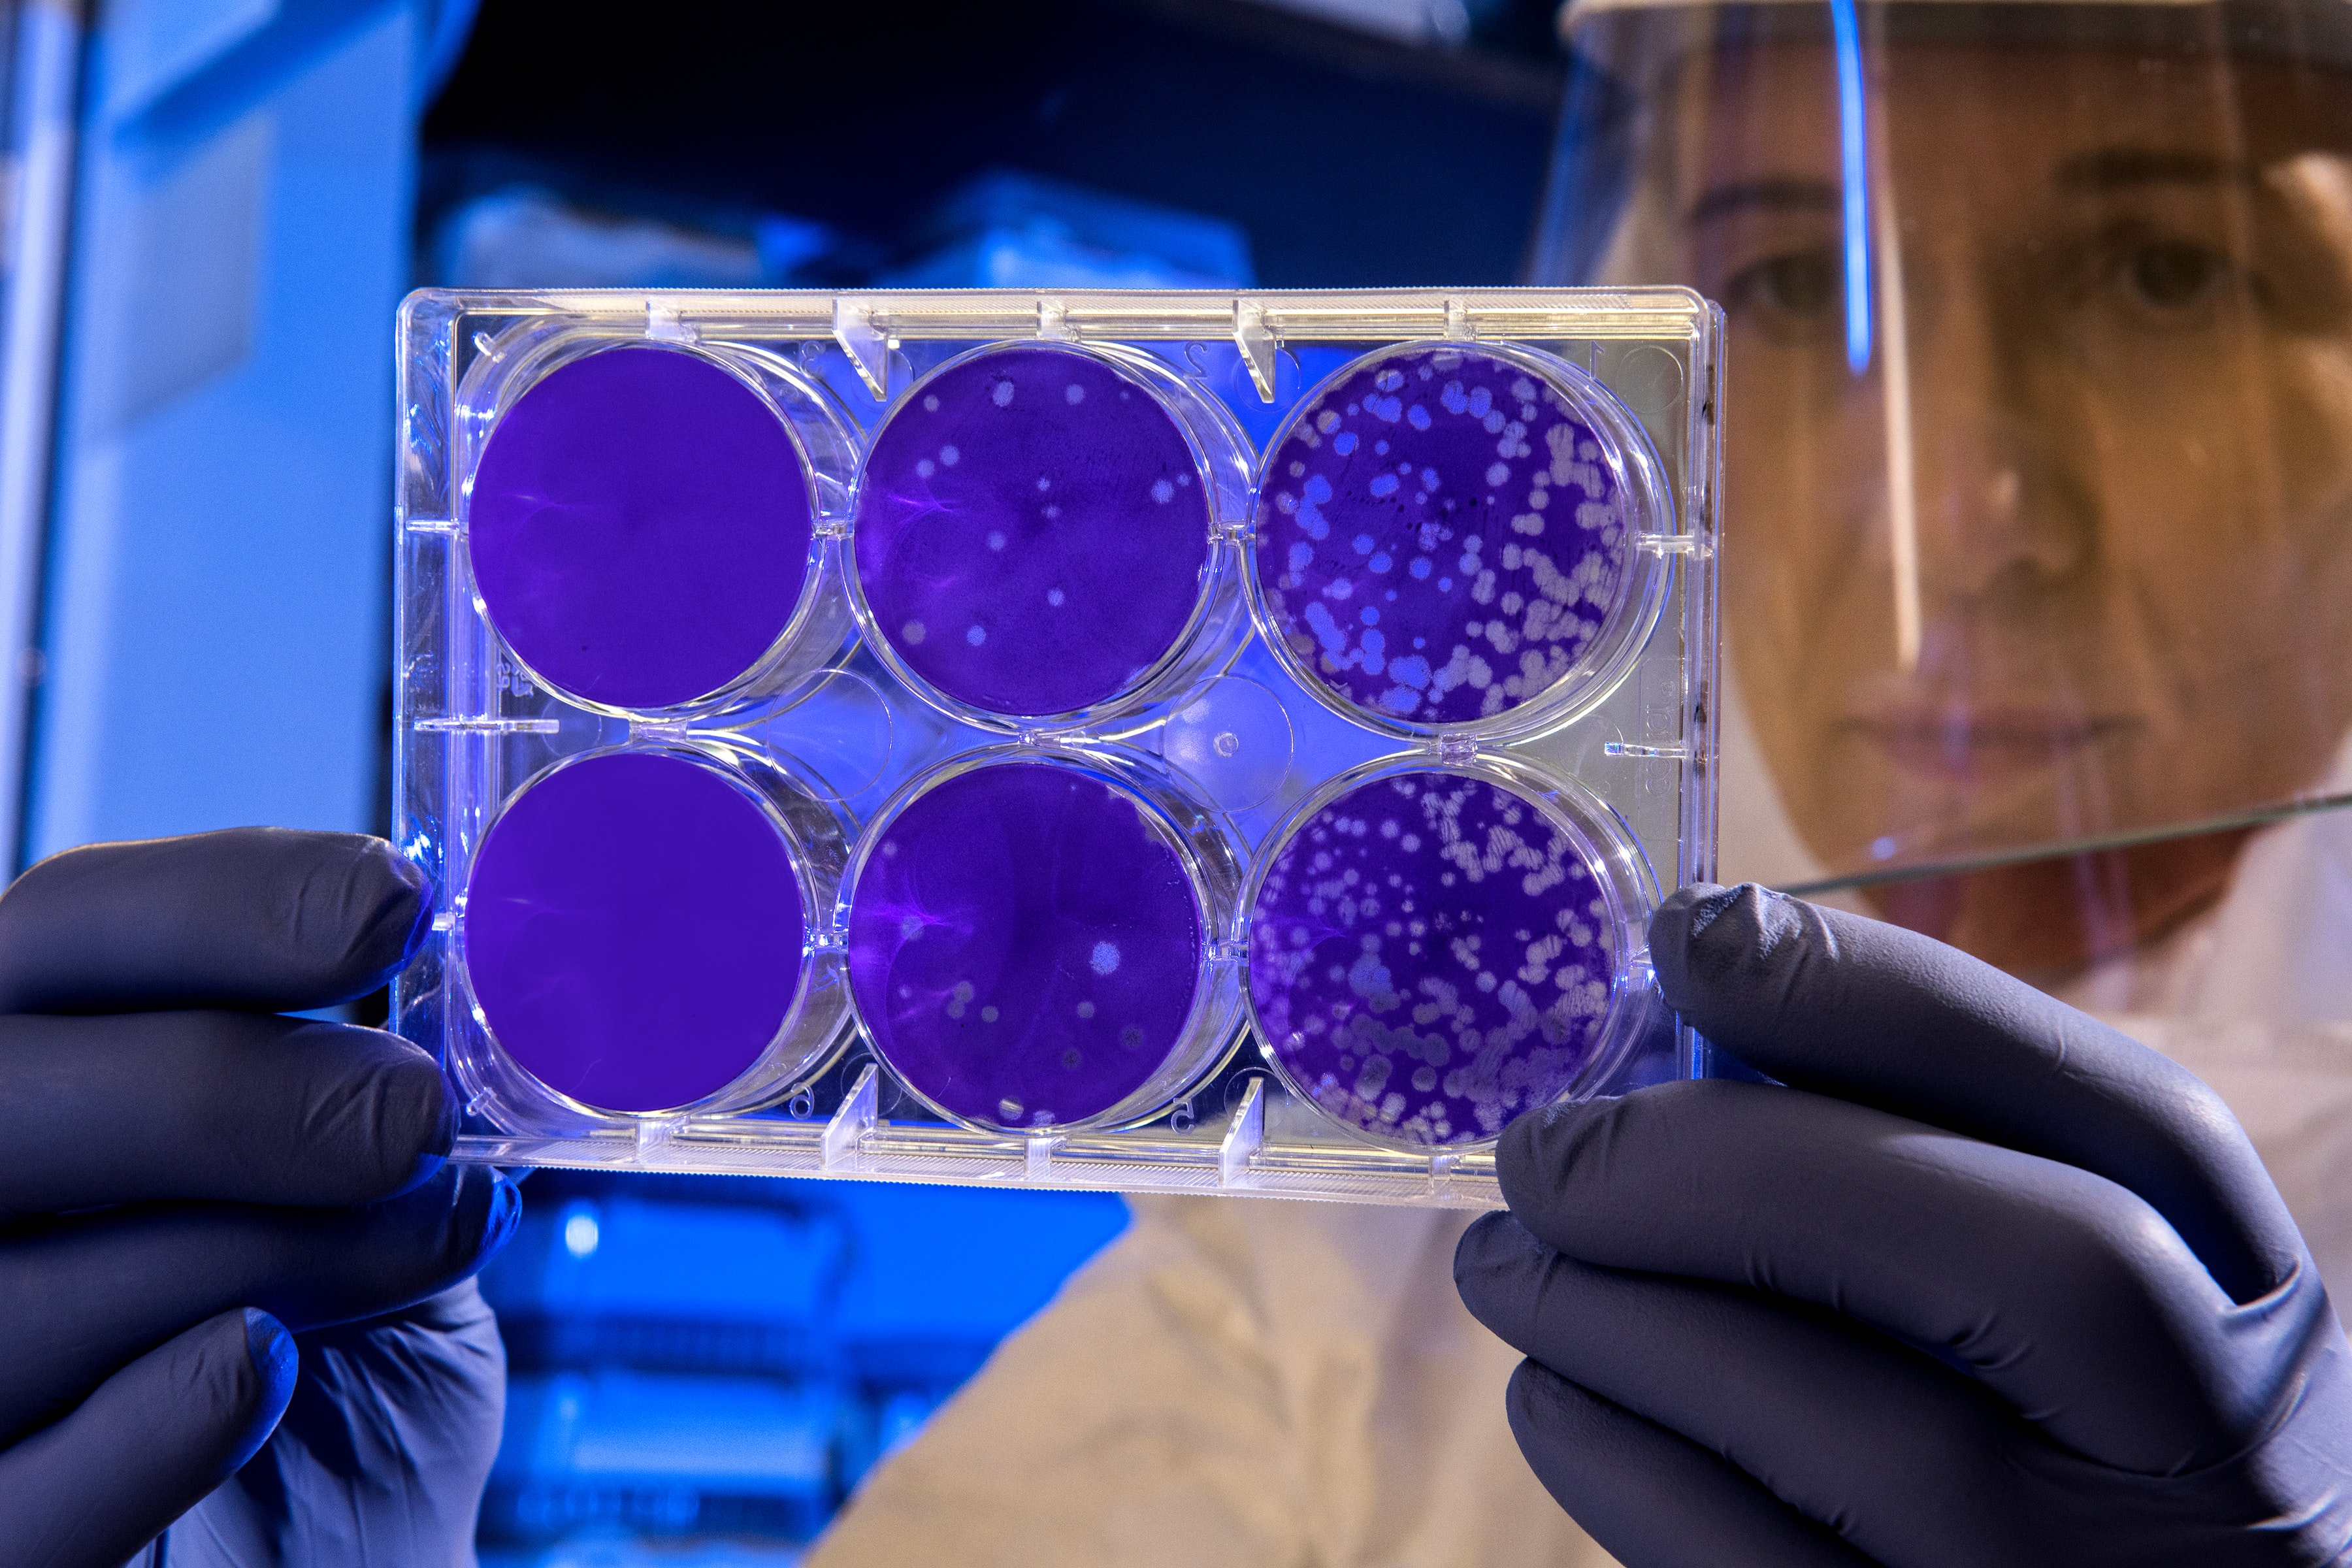
\includegraphics[width=0.8\linewidth]{images/unsplash} 

}

\caption{I found this image on unsplash.com by searching with the keyword "science"}\label{fig:unsplash}
\end{figure}

You can also upload GIFs which are animated images. These have become a very popular way to share moving images, particularly as a way to convey feelings and emotions. In fact, there's a whole genre of GIFs known as ``reaction GIFs''. But you can also use GIFs as a replacement for more conventional videos. If you're adding GIFs from another source, there's a 15MB limit when uploading from your desktop (5MB if uploading via mobile app)

You can also upload conventional videos via the Twitter website. Videos cannot be longer than 2 minutes and 20 seconds or larger than 512MB. There are a number of additional limitation when uploading videos via the Twitter website that you should also be aware of. Uploading videos via the Twitter mobile app is a lot less restrictive in terms of file formats, as you can upload both MOV and MP4 files.

\hypertarget{interacting-with-other-tweets}{%
\subsection{Interacting with other tweets}\label{interacting-with-other-tweets}}

When you see other tweets in your main feed, you can primarily interact with them four ways (liking, retweeting, replying, and sending via direct message), which I'm going to cover now.

\hypertarget{liking-tweets}{%
\subsection{Liking tweets}\label{liking-tweets}}

You can `like' a tweet by clicking on the little heart. This acknowledges both the to tweet author and to other people that you liked the tweet (e.g.~someone tweeted good news, and interesting article, or shared a funny meme). Keep in mind that when you like a tweet, this \emph{might} appear in the feed of people that follow you. You might also see tweets that people you follow have liked in your feed too.

Liking is also a useful way of acknoledging that you read a tweet that mentioned you. Remember, it's nice to respond to tweets that mention you, and this can help build you Twitter network, but don't feel an obligation to respond to every tweet. Sometimes a like is ok.

\hypertarget{retweeting}{%
\subsection{Retweeting}\label{retweeting}}

If you come accross a tweet that you think your followers would like, then you can use the Retweet function. When you click on the Retweet button, you'll get two options. The first option is a conventional retweet, which will appear in your follower's timeline. Your followers will also be able to see that you've retweeted the tweet. Here is an example of a retweet.

Tilting your head up makes you look more dominant, but less attractive https://t.co/L22Rq69l9T huh pic.twitter.com/5ZiJ9rgrAH

--- Neuroskeptic (\citet{Neuro_Skeptic}) March 4, 2020

The second option is to ``Retweet with comment''. This allows you to share the tweet, along with your comment above. This is a good way to describe \emph{why} you're retweeting a particular tweet.

If you're interested in science communication this episode is for you ⤵️ \#TeamTwitterThread https://t.co/rknRa0Al7Z

--- Dan Quintana (\citet{dsquintana}) March 2, 2020

\hypertarget{replying-to-tweets}{%
\subsection{Replying to tweets}\label{replying-to-tweets}}

One of the great things about twitter is that it makes it much easier to chat with people that are otherwise difficult to contact via email. One of the main reasons for this is that there's also no friction when composing a tweet. An email (usually) includes a salutation, some brief chit-chat, the actual question or comment, then a sign off. With twitter you just write the question or comment. In the following example, I'm replying to a tweet ``\citet{xieyihui}'', who quote-retweeted one of my tweets.

You've read my mind 😎 I hope to do one after I've had a little more experience with the package. I hadn't realised until using it how useful bookdown could be for technical documents!

--- Dan Quintana (\citet{dsquintana}) March 4, 2020

Replying to tweets is one of the best ways to build a network, as it helps you to establish your expertise in your topic area. All the usual tweeting options are also available for replies.

\hypertarget{direct-messages}{%
\subsection{Direct messages}\label{direct-messages}}

You can send private messages to other Twitter users. This is a useful feature if you want to ask a question, but would rather the question wasn't public. But keep in mind that you can only send direct messages to people that are following you or people that have opted in the recieve direct message from anyone.

\hypertarget{your-twitter-style}{%
\section{Your Twitter style}\label{your-twitter-style}}

\hypertarget{how-personal-should-you-tweets-be}{%
\subsection{How personal should you tweets be?}\label{how-personal-should-you-tweets-be}}

This is up to you, so share whatever you're confortable with. Some people like to keep their personal lives seperate from their academic lives, and others like to mix things up. One benefit of sharing some personal tweets is that it gives you a little more personality, but don't feel that you have to do this.

\hypertarget{finding-your-twitter-voice}{%
\subsection{Finding your twitter `voice'}\label{finding-your-twitter-voice}}

Just be yourself. Trying to be someone you're not on Twitter can be exhausting. Another aspect to consider is how ``professional'' your Twitter account should be. Some people think that you shouldn't tweet anything you wouldn't say in front of a live audience of your peers. I understand this sentiment, and realise that different fields have different conventions. But at the same time, you also need to think about the \emph{context} of twitter, which is typically more casual than doing a academic talk.

\hypertarget{using-a-psuedonym}{%
\subsection{Using a psuedonym}\label{using-a-psuedonym}}

Some academics would prefer to not use their real identities on Twitter, for various reasons. While not using a real identity can limit some of the benefits of Twitter, such as potential collaborations, a psuedonomous user will still reap several benefits from using Twitter, such as learning new tools, asking questions to other researchers, and testing new ideas.

\hypertarget{finding-people-to-follow}{%
\section{Finding people to follow}\label{finding-people-to-follow}}

There are various ways to find people to follow on Twitter. Try searching for some key words of interest, and have a look at the users behind these tweets. If you've found a few interesting accounts, have a look at who they're following. Over time, you'll find more accounts as you'll come across more retweets from accounts that you don't follow.

You will also see a ``Who to follow'' box next to your main feed on the desktop site. These are \emph{usually} good recommendations, but sometimes they provide some odd suggestions. Either way, these recommended users are worth checking out from time to time. These recommendations are based on the accounts the people you are following are interacting with and following themselves.

\hypertarget{one-month-twitter-plan}{%
\section{One-month twitter plan}\label{one-month-twitter-plan}}

It can be hard to get started, so here's a one-month plan that you can use. If you follow this plan, you'll get well on your way to building a Twitter network. Just remember that twitter should be fun. If doing this challenge feels like drudgery, then don't do it.

\hypertarget{tweet-at-least-once-every-weekday}{%
\subsection{Tweet at least once every weekday}\label{tweet-at-least-once-every-weekday}}

People are less likely to follow you if you're only send out a tweet whenever you publish a paper. By tweeting daily, you demonstrating that you're regularly participating. I covered the kind of things you can tweet in section XXX, but here's quick recap:

\begin{itemize}
\tightlist
\item
  Interesting tools you're using
\item
  Interesting papers you've come accross
\item
  Ask questions, tagging experts in your field (but don't go overboard tagging people)
\item
  Run a poll
\item
  Describe one of your new papers (or an old one)
\item
  Retweet someone else's tweet
\end{itemize}

\hypertarget{comment-on-someone-elses-tweet-at-least-once-every-weekday}{%
\subsection{Comment on someone else's tweet at least once every weekday}\label{comment-on-someone-elses-tweet-at-least-once-every-weekday}}

This could be as simple as saying, ``Thanks for the link, this was great!'', or a more in-depth comment on a tweet. Twitter provides incredible access to a massive community of scientists.

\hypertarget{what-to-tweet-about}{%
\chapter{What to tweet about}\label{what-to-tweet-about}}

So now you up to speed with the general mechanics of twitter, but should you actually tweet about? When talking to people new to Twitter, or who are hesitant to begin, I find that this is one of the biggest hurdles to overcome. But as soon as you realise that the \emph{process} of your work is just as interesting than as the \emph{output}, then things become much easier.

In my opinion, I think it's difficult to tweet \emph{too much}. In the early days of Twitter, were users didn't follow that many people, it was pretty easy to flood someone's timeline. But now, people tend to follow hundreds (sometimes thousands) of accounts, so this is harder to do. The upside of more tweets outweighs the downside a few people unfollowing you. You never know which tweets other people will find of interest.

Another important point to consider is that good tweets reduce friction and uncertaintly. For example, people are more likely to click on a link to a paper if they can read the abstract first. By including an image of an abstract in your tweet, people can quickly scan if the paper is worth downloading.

\hypertarget{some-example-tweets}{%
\section{Some example tweets}\label{some-example-tweets}}

\hypertarget{sharing-your-toolkit}{%
\subsection{Sharing your toolkit}\label{sharing-your-toolkit}}

We use several tools for our research everyday. Even if these tools seem commonplace to your, your followers will value learning about new ways to do their work. Here is an example of me tweeting about the \texttt{bookdown} R package, which I'm using to write this book

Starting to get the hang of the \{bookdown\} \#Rstats package, super impressed! Check out this package if you've ever wanted to put together a book, technical document, or long-form document https://t.co/5Wa4ISkYUG

--- Dan Quintana (\citet{dsquintana}) March 4, 2020

Notice that the link has been converted into a small image with information, which is called a Twitter card. This is a feature of more modern websites, which include Twitter card info in their underlying code. If your Tweeting from your phone, the twitter card will appear if its's available, as soon as you enter the link. This doesn't occur when tweeting from your desktop, but you can quickly check if there's a Twitter card associated with the link you're going to post on the Twitter \href{https://cards-dev.twitter.com/validator}{Card Validator} website.

\hypertarget{asking-a-question}{%
\subsection{Asking a question}\label{asking-a-question}}

Twitter can be a really good way to get advice. If you don't have many followers, you should also consider tagging experts that might know the answer (but don't spam people, so use this sparingly). Here's an example that I used, which was also used for researching this book.

I'm putting something together on twitter profile/bio pages for an upcoming talk. What do you think makes a `good' twitter profile, when it comes to images, text, web URL etc\ldots{}? What makes you think, ``Yeah, I'm going to follow them\ldots{}''?

--- Dan Quintana (\citet{dsquintana}) March 3, 2020

\hypertarget{sharing-memes}{%
\subsection{Sharing memes}\label{sharing-memes}}

Memes are fun, but also a good way to demonstrate knowledge and authority in your area. Here's an example that's fun, but also an opportunity to share expertise. Notice that this tweet was a quote retweet, so that people can see that I've put together a meme that someone else has used.

Hi, I'm a psychoneuroendocrinologist. You might know me from my smash hits: ``Don't Buy Oxytocin Online'', ``You Can't Measure Peripheral Blood Oxytocin Levels to Infer Brain Levels'', and ``Your Sample Size is Too Small'', OR my chart-topping ``Oxytocin Is Not the Cuddle Chemical'' https://t.co/gWdNe1quX0

--- Dan Quintana (\citet{dsquintana}) March 2, 2020

\hypertarget{sharing-videos}{%
\subsection{Sharing videos}\label{sharing-videos}}

You can include a video that up to two minutes and twenty seconds long to your tweet. In the following tweet, I've included a link to an eleven-minute instructional YouTube video. I can't show the entire video, so I've included a short preview to entice people to click on the link.

How to make a reproducible version of your \#Rstats analysis that can be run in any modern web browser, using \citet{_inundata}'s `holepunch' package + \citet{mybinderteam} Full screencast w/links {[}11 mins{]} 👉 https://t.co/5sjlN0iY4hPreview 👇 pic.twitter.com/SsX8qozMJ8

--- Dan Quintana (\citet{dsquintana}) August 15, 2019

While GIFs are a better option for very short videos (up to about 10 seconds), videos are better for longer clips. Here is a \href{https://twitter.com/dsquintana/status/1162002047794864128?s=20}{link to the tweet}, if you'd like to watch the actual video.

\hypertarget{a-commentary-on-a-peer-review}{%
\subsection{A commentary on a peer-review}\label{a-commentary-on-a-peer-review}}

Peer review is a task that most of us do, so you can take this opportunity to make a wider point about your research topic. For instance, I recently shared a point about power analysis using a peer-review I was conducting as an example. So let's break down this tweet (Figure \ref{fig:power}).

\begin{figure}

{\centering \includegraphics[width=0.8\linewidth]{images/power} 

}

\caption{A tweet discussing peer review}\label{fig:power}
\end{figure}

\begin{enumerate}
\def\labelenumi{\arabic{enumi}.}
\tightlist
\item
  I used a line break to clearly seperate the two parts of this tweet
\item
  The screenshot image is eye catching and conveys a lot of information
\item
  The `down arrow' emoji adds a tiny bit of flair
\item
  I tagged a tool that I mentioned (\citet{jamovistats}), so that followers could easily find out more
\item
  I numbered this tweet ``1/2'', to signal that this is a two-part tweet. My followers will see these two tweets back-to-back, but people who see this tweet as a retweet will release there's more
\end{enumerate}

Of course, if you're going to tweet about peer review you will need to keep things as anonomous as possible.

\hypertarget{tweeting-about-your-own-research-papers}{%
\subsection{Tweeting about your own research papers}\label{tweeting-about-your-own-research-papers}}

This is one of the most common tweets you'll see from scientists who aren't very active on Twitter. When a new paper is published, they'll log on, post the title of thier paper with a link to the paper, and then log off until their next paper is published. There are so many more types of tweets that you can do, but I'm going to walk through how you can life your game with these types of tweets.

\begin{enumerate}
\def\labelenumi{\arabic{enumi}.}
\item
  Add an image from the paper to go with the tweet.
  Have a look through the paper to see if there's a nice image that can be used. If there's no images, you can just take a screenshot of the abstract or a particularly interesting part of the paper. \href{https://evernote.com/products/skitch}{Skitch} is a handy app for screenshots, as you can easily annotate and highlight images.
\item
  Add a quote from the paper
  Find a striking quote from the paper to include in your tweet. You can either write this as text, or take a screenshot with and then highlight the quote.
\item
  Tag your co-authors and the journal, if they're on twitter.
  Co-authored papers are a team effort, so you should acknoledge your team
\item
  Add your own commentary of the paper
  If you're not including a quote, you should share why do you think the paper is interesting
\item
  Add a link to a non-paywalled version of the paper
  People might see the tweet, but not bother clicking on the link if they do not have institutional access to the journal. However, if you include a link to a preprint or a postprint\footnote{A preprint is a version of an article that is posted to a preprint repository before peer-review. Most journals allow you to submit papers that have been posted as preprints and do not consider this dual-publication. Check your journal's policies. A postprint is a version of paper that has undergone peer-review but has not been typeset. These are typically posted to author's personal or institutional websites. Postprints and are usually just a PDF version of the final Word document that was sent to the journal. Unlike preprints, journal policies vary regarding postprints, so it's best to check before uploading one.}
\end{enumerate}

In the following example of a paper I co-authored, I mention a summary of the results, tag my co-authors on Twitter, include a postprint of the article, and a figure from the artile (Figure \ref{fig:new-paper-own}).

\begin{figure}

{\centering \includegraphics[width=0.8\linewidth]{images/new_paper_own} 

}

\caption{Announcing your new paper}\label{fig:new-paper-own}
\end{figure}

While single tweets announcing new papers can be an effective way to share your new work, I think a thread (see section X) does a better job.

\hypertarget{tweeting-about-other-peoples-research-papers}{%
\subsection{Tweeting about other people's research papers}\label{tweeting-about-other-peoples-research-papers}}

There are only so many articles that you can co-author. So in addition, you should also share papers that you find interesting.

Below is an example of tweeting a link to a new paper, in which I added an image and quote from the paper, and mentioned the lead author and the journal that it was published in (Figure \ref{fig:paper-mention}).

\begin{figure}

{\centering \includegraphics[width=0.8\linewidth]{images/paper_mention} 

}

\caption{A tweet mentioning a new paper}\label{fig:paper-mention}
\end{figure}

\hypertarget{intermediate-twitter-skills}{%
\chapter{Intermediate twitter skills}\label{intermediate-twitter-skills}}

Here are a few ways that you can lift your Twitter game now that you've got some experience.

\hypertarget{pinning-a-tweet-to-your-profile}{%
\section{Pinning a tweet to your profile}\label{pinning-a-tweet-to-your-profile}}

Once you've got a few tweets under your belt, you should `pin' one of these tweets to the top of you profile. A pinned tweet will be the first tweet that someone sees when they visit your profile, so use this wisely. Here are some ideas of the types of tweets you should consider pinning to your profile:

\begin{itemize}
\tightlist
\item
  Your latest paper
\item
  Your most important paper
\item
  Information about an upcoming talk
\item
  A summary of your current research project
\item
  An announcement for research participant recruitment
\end{itemize}

As for me, I tend to choose my most important paper at the time. This works, because these tweets continue to get likes and retweets long after I post them originally.

\hypertarget{bookmarking-tweets}{%
\section{Bookmarking tweets}\label{bookmarking-tweets}}

While some people like tweets as way to bookmark them for later use, Twitter does have a specific bookmarking feature. Just click on the share button under a tweet, then click on ``Add Tweet to Bookmarks'' (Figure \ref{fig:bookmark}).

\begin{figure}

{\centering \includegraphics[width=0.8\linewidth]{images/bookmark} 

}

\caption{Bookmarking tweets}\label{fig:bookmark}
\end{figure}

This is a handy feature for when you come across a tweet with a link to an intersting paper, for instance, but you don't have the time now to read it.

\hypertarget{hashtags}{%
\section{Hashtags}\label{hashtags}}

These are useful for categorizing your tweets. One example of hashtag use is that they can organise communities of likeminded people. The \#PhDchat hashtag is a community of PhD students who often post questions and support for the PhD student community (Figure \ref{fig:hashtag}).

\begin{figure}

{\centering \includegraphics[width=0.8\linewidth]{images/hashtag} 

}

\caption{Tagging users in photos.}\label{fig:hashtag}
\end{figure}

Hashtags are also useful for organising tweets related to a specific event, like a conference. Many conferences now announce their `official' hashtag that should be used for tweets related to a conference.

\hypertarget{images}{%
\section{Images}\label{images}}

When you post your images, you can tag Twitter usernames in your images. After adding your image, click on ``Tag people'' (Figure \ref{fig:tag}).

\begin{figure}

{\centering \includegraphics[width=0.8\linewidth]{images/tag} 

}

\caption{Tagging users in photos.}\label{fig:tag}
\end{figure}

Tagging photos has a few advantages. First, it saves you a few characters in your tweet as you tag people in the photo instead. Anyone that you tag will be notified that they've been included in a photo. You don't have to use this feature for tagging pictures of people. For example, you can post a screenshot of the abstract of a new paper and tag the co-authors of your paper.

\hypertarget{twitter-polls}{%
\section{Twitter polls}\label{twitter-polls}}

If you're reading this, you're probably a scientists, so should understand that Twitter polls are by no means scientific. However, they still provide \emph{some} information and provide a fun alternative to typical text tweets(Figure \ref{fig:poll}).

\begin{figure}

{\centering \includegraphics[width=0.8\linewidth]{images/poll} 

}

\caption{A twitter poll}\label{fig:poll}
\end{figure}

To improve data quality, people sometimes include a ``Show me the data'' option. This means that people who would like to see he results but don't want to particpate in the pool can select this. You can also set how long the poll should.

Polls can sometimes start an intersting discussion around the subject of the poll, so consider using this as a conversation starter.

\hypertarget{sharing-tweets-by-copying-thier-link}{%
\section{Sharing tweets by copying thier link}\label{sharing-tweets-by-copying-thier-link}}

As well as retweeting tweets, you can also share them by sharing the link to the tweet.

\hypertarget{advanced-twitter-skills}{%
\chapter{Advanced Twitter skills}\label{advanced-twitter-skills}}

\hypertarget{twitter-threads}{%
\section{Twitter threads}\label{twitter-threads}}

You can't say a lot in a 280-character tweet, but with a thread you can connect a series of tweets together to say a lot. In principle, there is no limit to how many tweets can go in a thread, however, Twitter will only let you post 20 consecutive tweets in a single instance. I think this is a sensible limit for a thread, but you can always add additional tweets after you've posted your first 20 if you like.

\hypertarget{using-a-twitter-thread-to-announce-a-new-paper}{%
\subsection{Using a twitter thread to announce a new paper}\label{using-a-twitter-thread-to-announce-a-new-paper}}

Threads are a great way to announce a new paper, as you can say much more than if you were posting a single tweet. To demonstrate, I've selectedeight tweets out of a twenty-five-tweet thread I used to summarise an important paper. Let's start with the first figure. Tweet A is the introduction, which includes a link to the actual paper and four images from the paper. I alos tagged the journal, who is active on Twitter, so that they could be notified of the tweet and hopefully retweet it (they did).

Tweet B is one of my paper background tweets, which gives a little context as to why I did the study. This striking image is prominent and a link is included if people want to read more.

Tweet C explains the story behind the paper idea and acknowledges the team behind the project. I also tag the source of the data and my co-authors

Tweet D covers some of the methods for our analysis

\hypertarget{making-your-own-gifs}{%
\section{Making your own GIFs}\label{making-your-own-gifs}}

GIFs get a lot of attention. Instead of just posting a static image of paper, you can create a video scrolling through your paper. Of course, you could post this as a video, but people often expect audio when they come accross a video. GIFs don't have audio and continually loop.

\hypertarget{getting-your-tweet-back-in-the-feed-again}{%
\section{Getting your tweet back in the feed again}\label{getting-your-tweet-back-in-the-feed-again}}

No matter where you are in the world, some of your followers will be asleep when you tweet. This means that they might miss your tweet. But there are ways to re-introduce your tweets again

\begin{enumerate}
\def\labelenumi{\arabic{enumi}.}
\item
  Retweeting your onw tweet. I would keep this to a absolute minimum, as this is the digital equivalent of patting yourself on the back.
\item
  Replying to your own tweet with an additional tweet
\end{enumerate}

\hypertarget{sharing-your-replies}{%
\section{Sharing your replies}\label{sharing-your-replies}}

If you've written a reply to someone's tweet, the only time it will appear in someone else's feed is if they follow both you and the person you replied to, or if the twitter algorithm somehow pushes this tweet into people's feed if it's produced a lot of likes or retweets. However, if you want more people to see it, you can retweet that particular reply tweet

\hypertarget{the-darkside-of-twitter}{%
\chapter{The darkside of Twitter}\label{the-darkside-of-twitter}}

So far I've covered all the benefits of Twitter. However, not everyone always has a positive experience on the platform. There are three main potential downsides to Twitter that I'm going to cover in this section.

\hypertarget{annoying-twitter-users-or-topics}{%
\section{Annoying twitter users or topics}\label{annoying-twitter-users-or-topics}}

There might be some situations where people are tweeting a lot, such as when they're tweeting updates from a conference. In these situations, you can mute specific users so they don't appear in your feed. They won't know that you've muted them and you're still following them. You can do this by clicking on the ``more'' button (the circle with three open circles) on a user's profile (Figure \ref{fig:mute}).

\begin{figure}

{\centering \includegraphics[width=0.8\linewidth]{images/mute} 

}

\caption{Muting a user}\label{fig:mute}
\end{figure}

You can also mute specific topics appearing in your times, for a set period of time (or forever) by adjusting your settings (Figure \ref{fig:mute-word}).

\begin{figure}

{\centering \includegraphics[width=0.8\linewidth]{images/mute_word} 

}

\caption{Muting a keyword}\label{fig:mute-word}
\end{figure}

\hypertarget{dealing-with-abusive-or-harmful-tweets}{%
\section{Dealing with abusive or harmful tweets}\label{dealing-with-abusive-or-harmful-tweets}}

While not everyone has experienced harmful tweets, it is important to acknowldege that are many cases of harassment and verbal abuse in the Twitter science community. This will probably not be a regular experience for you, but it \emph{could} happen.

You can block accounts, which means they can't follow you or interact with you. Keep in mind that if they log out of their account which was blocked, they can see your tweets (if they're public). But they can no longer interact with you.

You can also report abusive or harmful tweets (or accounts) to Twitter, by following \href{https://help.twitter.com/en/safety-and-security/report-abusive-behavior}{these instructions}.

\hypertarget{spending-too-much-time-on-twitter}{%
\section{Spending too much time on Twitter}\label{spending-too-much-time-on-twitter}}

Twitter is designed to hold your attention for as long as possible, so it's no suprise that it can become addictive. The constant flow of new information and the intermittent reward of likes, retweets, and new followers makes it really easy to get hooked. It wouldn't be this popular if it wasn't fun. This can become a problem, because if you're spending too much time on the platform then you'll have no work to share.

There's also desktop software available, like \href{https://selfcontrolapp.com/}{\emph{SelfControl}} (MacOS) and \href{https://getcoldturkey.com/pricing/}{\emph{Cold Turkey}} (MacOS and Windows), which can block distracting websites, like Twitter. You may want to set this for smaller blocks or for entire days. Personally, I work in periods of forty minutes, in which I block all distracting websites. I take a 10-20 minute break between work sessions, and that's when I usually check Twitter.

\bibliography{book.bib,packages.bib}


\end{document}
